

\mode<presentation>
{
  \usetheme{boxes}
  %\useoutertheme{infolines}
  % með efnisyfirliti: Szeged, Frankfurt 
  % án efnisyfirlits: Pittsburgh
  % áhugavert: CambridgeUS, Boadilla
  %\setbeamercovered{transparent} %gegnsætt
  \setbeamercovered{invisible}

\defbeamertemplate*{footline}{infolines theme}
{
  \leavevmode%
  \hbox{%
  \begin{beamercolorbox}[wd=.333333\paperwidth,ht=2.25ex,dp=1ex,center]{author in head/foot}%
  %  \usebeamerfont{author in head/foot}\insertshortauthor~~\beamer@ifempty{\insertshortinstitute}{}{(\insertshortinstitute)}
  \end{beamercolorbox}%
  \begin{beamercolorbox}[wd=.333333\paperwidth,ht=2.25ex,dp=1ex,center]{title in head/foot}%
   % \usebeamerfont{title in head/foot}\insertshorttitle
  \end{beamercolorbox}%
  \begin{beamercolorbox}[wd=.333333\paperwidth,ht=2.25ex,dp=1ex,right]{date in head/foot}%
    %\usebeamerfont{date in head/foot}\insertshortdate{}\hspace*{2em}
    \insertshortlecture.\insertframenumber{} / \insertshortlecture.\inserttotalframenumber\hspace*{2ex} 
  \end{beamercolorbox}}%
  \vskip0pt%
}
\resetcounteronoverlays{rtaskno} %Does not increase counter rtaskno on \pause in beamer


}


\usepackage[english,icelandic]{babel}
\usepackage[utf8]{inputenc}
\usepackage{t1enc}
\usepackage{graphicx}
\usepackage{amsmath}
\usepackage{amssymb}
\usepackage{mathrsfs}
\usepackage{verbatim}
\usepackage{esint}


% RAGNAR SIGURÐSSON
%\usepackage[T1]{fontenc} 
%\usepackage[icelandic]{babel}
\usepackage{latexsym,amssymb,amsmath}
%\usepackage[utf8]{inputenc}
%\usepackage{graphicx}
\usepackage{epstopdf}
\usepackage{verbatim}
\usepackage{array,tabularx,arydshln}
\setbeamertemplate{theorems}[numbered]


\newtheorem{setning}{Setning}
\newtheorem{hjalpar}{Hjálparsetning}
\theoremstyle{definition}
\newtheorem{rithattur}{Ritháttur}
\newtheorem{skilgreining}{Skilgreining}
\newtheorem{daemi}{Dæmi}
\newtheorem{ath}{Athugasemd}

\newcommand\Wider[2][3em]{%
\makebox[\linewidth][c]{%
  \begin{minipage}{\dimexpr\textwidth+#1\relax}
  \raggedright#2
  \end{minipage}%
  }%
}

%counter used for blocks
\newcounter{rtaskno}
\DeclareRobustCommand{\rtask}[1]{%
   \refstepcounter{rtaskno}%
    \thertaskno\label{#1}}

\newcommand{\C}{{\mathbb  C}}
\newcommand{\Z}{{\mathbb Z}}
\newcommand{\R}{{\mathbb  R}}
\newcommand{\N}{{\mathbb  N}}
\newcommand{\Q}{{\mathbb Q}}
\renewcommand{\phi}{\varphi}
\renewcommand{\epsilon}{\varepsilon}
\newcommand{\p}{{\partial}}
\renewcommand{\d}{{\partial}}

% RAGNAR SIGURÐSSON
\newcommand{\nin}{\mbox{$\;\not\in\;$}}
\newcommand{\dive}{\mbox{${\rm\bf div\,}$}}
\newcommand{\curl}{\mbox{${\rm\bf curl\,}$}}
\newcommand{\grad}{\mbox{${\rm\bf grad\,}$}}
\newcommand{\spann}{\mbox{${\rm Span}$}}
\newcommand{\tr}{\mbox{${\rm tr}$}}
\newcommand{\rank}{\mbox{${\rm rank}$}}
\newcommand{\image}{\mbox{${\rm image}$}}
\newcommand{\nullity}{\mbox{${\rm null}$}}
\newcommand{\proj}{\mbox{${\rm proj}$}}
\newcommand{\id}{\mbox{${\rm id}$}}
%\newcommand{\R}{\mbox{${\bf R}$}}
%\newcommand{\C}{\mbox{${\bf C}$}}
\newcommand{\Rn}{\mbox{${\bf R}^n$}}
\newcommand{\Rm}{\mbox{${\bf R}^m$}}
\newcommand{\Rk}{\mbox{${\bf R}^k$}}
\newcommand{\Av}{\mbox{${\bf A}$}}
\newcommand{\av}{\mbox{${\bf a}$}}
\newcommand{\uv}{\mbox{${\bf u}$}}
\newcommand{\vv}{\mbox{${\bf v}$}}
\newcommand{\wv}{\mbox{${\bf w}$}}
\newcommand{\xv}{\mbox{${\bf x}$}}
\newcommand{\zv}{\mbox{${\bf z}$}}
\newcommand{\yv}{\mbox{${\bf y}$}}
\newcommand{\bv}{\mbox{${\bf b}$}}
\newcommand{\cv}{\mbox{${\bf c}$}}
\newcommand{\dv}{\mbox{${\bf d}$}}
\newcommand{\ev}{\mbox{${\bf e}$}}
\newcommand{\fv}{\mbox{${\bf f}$}}
\newcommand{\gv}{\mbox{${\bf g}$}}
\newcommand{\hv}{\mbox{${\bf h}$}}
\newcommand{\iv}{\mbox{${\bf i}$}}
\newcommand{\jv}{\mbox{${\bf j}$}}
\newcommand{\kv}{\mbox{${\bf k}$}}
\newcommand{\pv}{\mbox{${\bf p}$}}
\newcommand{\nv}{\mbox{${\bf n}$}}
\newcommand{\qv}{\mbox{${\bf q}$}}
\newcommand{\rv}{\mbox{${\bf r}$}}
\newcommand{\sv}{\mbox{${\bf s}$}}
\newcommand{\tv}{\mbox{${\bf t}$}}
\newcommand{\ov}{\mbox{${\bf 0}$}}
\newcommand{\Fv}{\mbox{${\bf F}$}}
\newcommand{\Gv}{\mbox{${\bf G}$}}
\newcommand{\Uv}{\mbox{${\bf U}$}}
\newcommand{\Nv}{\mbox{${\bf N}$}}
\newcommand{\Hv}{\mbox{${\bf H}$}}
\newcommand{\Ev}{\mbox{${\bf E}$}}
\newcommand{\Sv}{\mbox{${\bf S}$}}
\newcommand{\Tv}{\mbox{${\bf T}$}}
\newcommand{\Bv}{\mbox{${\bf B}$}}
\newcommand{\Oa}{\mbox{$(0,0)$}}
\newcommand{\Ob}{\mbox{$(0,0,0)$}}
\newcommand{\Onv}{\mbox{$[0,0,\ldots,0]$}}
\newcommand{\an}{\mbox{$(a_1,a_2, \ldots,a_n)$}}
\newcommand{\xn}{\mbox{$(x_1,x_2, \ldots,x_n)$}}
\newcommand{\xnv}{\mbox{$[x_1,x_2, \ldots,x_n]$}}
\newcommand{\vnv}{\mbox{$[v_1,v_2, \ldots,v_n]$}}
\newcommand{\wnv}{\mbox{$[w_1,w_2, \ldots,w_n]$}}
\newcommand{\tvint}{\int\!\!\!\int}
\newcommand{\thrint}{\int\!\!\!\int\!\!\!\int}
\renewcommand{\ast}{{\operatorname{\text{astand}}}}


\usepackage{caption}
%\usepackage{pgfpages}
% \pgfpagesuselayout{2 on 1}[a4paper,border shrink=5mm]

\def\lecturename{Stærðfræðigreining IIB}
\title{\insertlecture}
\author{Sigurður Örn Stefánsson, \href{mailto:sigurdur@hi.is}{sigurdur@hi.is}}
\institute
{
  Verkfræði- og náttúruvísindasvið\\
  Háskóli Íslands
}
\subtitle{Stærðfræðigreining IIB, STÆ205G}
%\subject{\lecturename}

\mode<article>
{
	\usepackage[colorlinks=false,
	pdfauthor={Sigurður Örn Stefánson},
	%pdftitle={Töluleg greining}
	]{hyperref}
  %\usepackage{times}
  %\usepackage{mathptmx}
  \usepackage[left=1.5cm,right=4cm,top=1.5cm,bottom=3cm]{geometry}
}

% Beamer version theme settings

%\useoutertheme[height=0pt,width=2cm,right]{sidebar}
%\usecolortheme{rose,sidebartab}
%\useinnertheme{circles}
%\usefonttheme[only large]{structurebold}


\setbeamercolor{sidebar right}{bg=black!15}
\setbeamercolor{structure}{fg=blue}
\setbeamercolor{author}{parent=structure}

\setbeamerfont{title}{series=\normalfont,size=\LARGE}
\setbeamerfont{title in sidebar}{series=\bfseries}
\setbeamerfont{author in sidebar}{series=\bfseries}
\setbeamerfont*{item}{series=}
\setbeamerfont{frametitle}{size=}
\setbeamerfont{block title}{size=\small}
\setbeamerfont{subtitle}{size=\normalsize,series=\normalfont}


\setbeamertemplate{sidebar right}
{
  {\usebeamerfont{title in sidebar}%
    \vskip1.5em%
    \hskip3pt%
    \usebeamercolor[fg]{title in sidebar}%
    \insertshorttitle[width=2cm-6pt,center,respectlinebreaks]\par%
    \vskip1.25em%
  }%
  {%
    \hskip3pt%
    \usebeamercolor[fg]{author in sidebar}%
    \usebeamerfont{author in sidebar}%
    \insertshortauthor[width=2cm-2pt,center,respectlinebreaks]\par%
    \vskip1.25em%
  }%
  \hbox to2cm{\hss\insertlogo\hss}
  \vskip1.25em%
  \insertverticalnavigation{2cm}%
  \vfill
  \hbox to 2cm{\hfill\usebeamerfont{subsection in
      sidebar}\strut\usebeamercolor[fg]{subsection in
      sidebar}\insertshortlecture.\insertframenumber\hskip5pt}%
  \vskip3pt%
}%

\setbeamertemplate{title page}
{
  \vbox{}
  \vskip1em
  %{\huge Kapitel \insertshortlecture\par}
  {\usebeamercolor[fg]{title}\usebeamerfont{title}\inserttitle\par}%
  \ifx\insertsubtitle\@empty%
  \else%
    \vskip0.25em%
    {\usebeamerfont{subtitle}\usebeamercolor[fg]{subtitle}\insertsubtitle\par}%
  \fi%     
  \vskip1em\par
  %Vorlesung \emph{\lecturename}\ vom 
  \insertdate\par
  \vskip0pt plus1filll
  \leftskip=0pt plus1fill\insertauthor\par
  \insertinstitute\vskip1em
}

%\logo{\includegraphics[width=2cm]{beamerexample-lecture-logo.pdf}}



% Article version layout settings

\mode<article>

\makeatletter
\def\@listI{\leftmargin\leftmargini
  \parsep 0pt
  \topsep 5\p@   \@plus3\p@ \@minus5\p@
  \itemsep0pt}
\let\@listi=\@listI


\setbeamertemplate{frametitle}{\paragraph*{\insertframetitle\
    \ \small\insertframesubtitle}\ \par
}
\setbeamertemplate{frame end}{%
  \marginpar{\scriptsize\hbox to 1cm{\sffamily%
      \hfill\strut\insertshortlecture.\insertframenumber}\hrule height .2pt}}
\setlength{\marginparwidth}{1cm}
\setlength{\marginparsep}{1.5cm}

\def\@maketitle{\makechapter}

\def\makechapter{
  \newpage
  \null
  \vskip 2em%
  {%
    \parindent=0pt
    \raggedright
    \sffamily
    \vskip8pt
    %{\fontsize{36pt}{36pt}\selectfont Kapitel \insertshortlecture \par\vskip2pt}
    {\fontsize{24pt}{28pt}\selectfont \color{blue!50!black} \insertlecture\par\vskip4pt}
    {\Large\selectfont \color{blue!50!black} \insertsubtitle, \@date\par}
    \vskip10pt

    \normalsize\selectfont \@author\par\vskip1.5em
    %\hfill BLABLA
  }
  \par
  \vskip 1.5em%
}

\let\origstartsection=\@startsection
\def\@startsection#1#2#3#4#5#6{%
  \origstartsection{#1}{#2}{#3}{#4}{#5}{#6\normalfont\sffamily\color{blue!50!black}\selectfont}}

\makeatother

\mode
<all>



% Typesetting Listings

\usepackage{listings}
\lstset{language=Java}

\alt<presentation>
{\lstset{%
  basicstyle=\footnotesize\ttfamily,
  commentstyle=\slshape\color{green!50!black},
  keywordstyle=\bfseries\color{blue!50!black},
  identifierstyle=\color{blue},
  stringstyle=\color{orange},
  escapechar=\#,
  emphstyle=\color{red}}
}
{
  \lstset{%
    basicstyle=\ttfamily,
    keywordstyle=\bfseries,
    commentstyle=\itshape,
    escapechar=\#,
    emphstyle=\bfseries\color{red}
  }
}



% Common theorem-like environments

\theoremstyle{definition}
\newtheorem{exercise}[theorem]{\translate{Exercise}}




% New useful definitions:

\newbox\mytempbox
\newdimen\mytempdimen

\newcommand\includegraphicscopyright[3][]{%
  \leavevmode\vbox{\vskip3pt\raggedright\setbox\mytempbox=\hbox{\includegraphics[#1]{#2}}%
    \mytempdimen=\wd\mytempbox\box\mytempbox\par\vskip1pt%
    \fontsize{3}{3.5}\selectfont{\color{black!25}{\vbox{\hsize=\mytempdimen#3}}}\vskip3pt%
}}

\newenvironment{colortabular}[1]{\medskip\rowcolors[]{1}{blue!20}{blue!10}\tabular{#1}\rowcolor{blue!40}}{\endtabular\medskip}

\def\equad{\leavevmode\hbox{}\quad}

\newenvironment{greencolortabular}[1]
{\medskip\rowcolors[]{1}{green!50!black!20}{green!50!black!10}%
  \tabular{#1}\rowcolor{green!50!black!40}}%
{\endtabular\medskip}


\begin{document}

%x
\section{Hagnýting hlutafleiðujafna}

\subsection{Útgildi} 

\subsubsection{Skilgreining \arabic{mycount}}\stepcounter{mycount}
 Látum $f$ vera fall af tveim breytum
skilgreint á mengi ${\cal D}(f)$.  

\medskip
Sagt er að $f$ hafi {\em \color{red} staðbundið
  lággildi} (e.~local minimum) í punkti $(a,b)$ ef til er tala $r>0$ þannig að 
$f(a,b)\leq f(x,y)$ fyrir alla punkta $(x,y)\in B_r(a,b)\cap{\cal
  D}(f)$.

\medskip
Sagt er að $f$ hafi {\em \color{red} staðbundið
  hágildi}  (e.~local maximum) í punkti $(a,b)$ ef til er tala $r>0$ þannig að 
$f(a,b)\geq f(x,y)$ fyrir alla punkta $(x,y)\in B_r(a,b)\cap{\cal
  D}(f)$.

\medskip
Í þeim punktum þar sem $f$ tekur annað hvort staðbundið lággildi eða
staðbundið hágildi er sagt að $f$ hafi {\em \color{red} staðbundið útgildi}
(e.~local extreme). 


\medskip
Ef $f(a,b)\leq f(x,y)$ fyrir alla punkta $(x,y)\in {\cal D}(f)$ þá er
sagt að $f$ taki {\em \color{red} lægsta gildi} í $(a,b)$ (e.~global minimum).
Ef $f(a,b)\geq f(x,y)$ fyrir alla punkta $(x,y)\in {\cal D}(f)$ þá er
sagt að $f$ taki {\em \color{red} hæsta gildi} í $(a,b)$ (e.~global maximum).




%x


\subsection{Staðbundið útgildi} 

\subsubsection{Upprifjun  \arabic{mycount}}\stepcounter{mycount}
   Látum $f$ vera fall af einni breytu
skilgreint á mengi ${\cal D}(f)\subseteq \R$.  Ef fallið $f$ hefur
staðbundið útgildi í punkti $a$ þá gildir eitt af þrennu um $a$:

\begin {enumerate}
 \item $f'(a)=0$. \qquad (punkturinn $a$ kallast {\em \color{red} stöðupunktur} $f$).
 \item Afleiðan $f'(a)$ er ekki skilgreind.
 \item   Punkturinn $a$ er jaðarpunktur ${\cal D}(f)$.
\end {enumerate}




%x

\subsubsection{Setning  \arabic{mycount}}\stepcounter{mycount}
 Látum $f$ vera fall af tveim breytum
skilgreint á mengi ${\cal D}(f)\subseteq \R^2$.  Ef fallið $f$ hefur
staðbundið útgildi í punkti $(a,b)$ þá gildir eitt af þrennu um $a$
\begin {enumerate}
 \item  $\nabla f(a,b)=\ov$. \qquad (punkturinn $(a,b)$ kallast {\em \color{red}
     stöðupunktur} $f$) 
\item Stigullinn $\nabla f(a,b)$ er ekki skilgreindur.
\item Punkturinn $(a,b)$ er jaðarpunktur ${\cal D}(f)$.
\end {enumerate}




%x

  Dæmi: Föll skilgreind á svæðinu $-0.5 \leq x \leq 0.5$,  $-0.5 \leq y \leq 0.5$. Hvar eru staðbundin hágildi?
  \begin{figure}[!h]
        \centering
        \begin{minipage}{.5\textwidth}
            \centering
            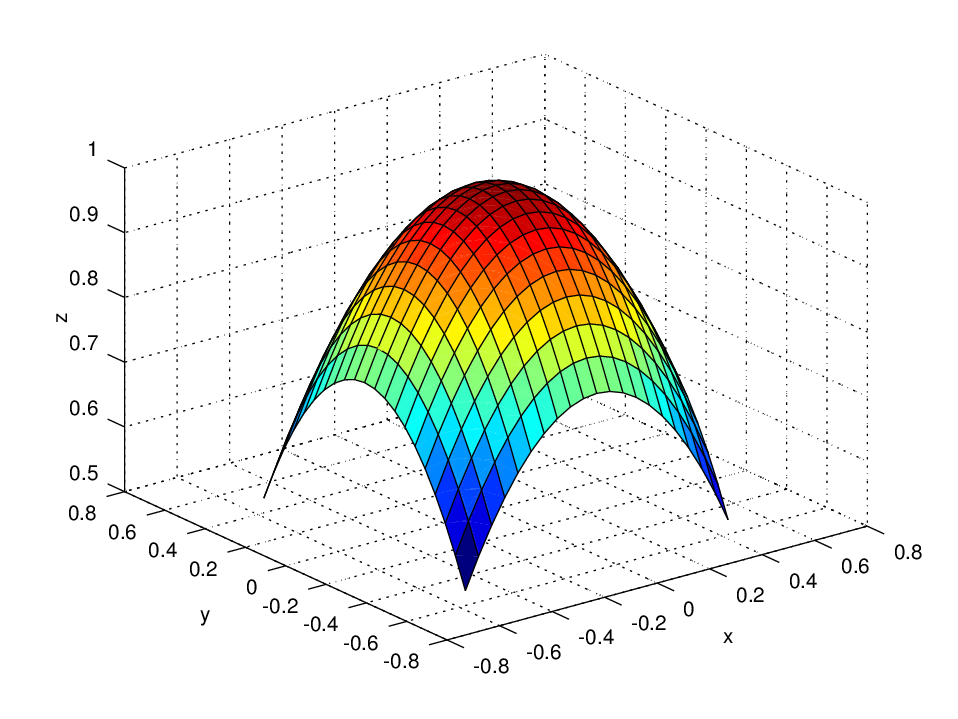
\includegraphics[width=.8\linewidth]{peak_smooth.png}
            \caption*{$z = f(x,y) = 1-x^2-y^2$.}
        \end{minipage}%
        \begin{minipage}{.5\textwidth}
            \centering
            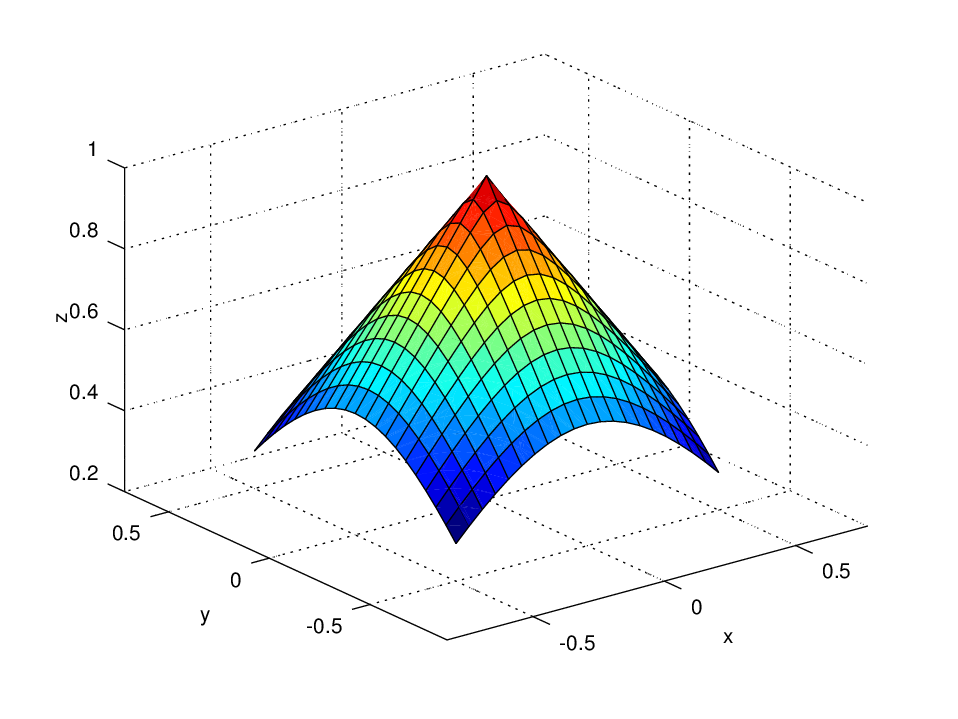
\includegraphics[width=.8\linewidth]{peak.png}
            \caption*{$z = f(x,y) = 1-\sqrt{x^2+y^2}$.}
        \end{minipage}
        \begin{minipage}{.5\textwidth}
            \centering
            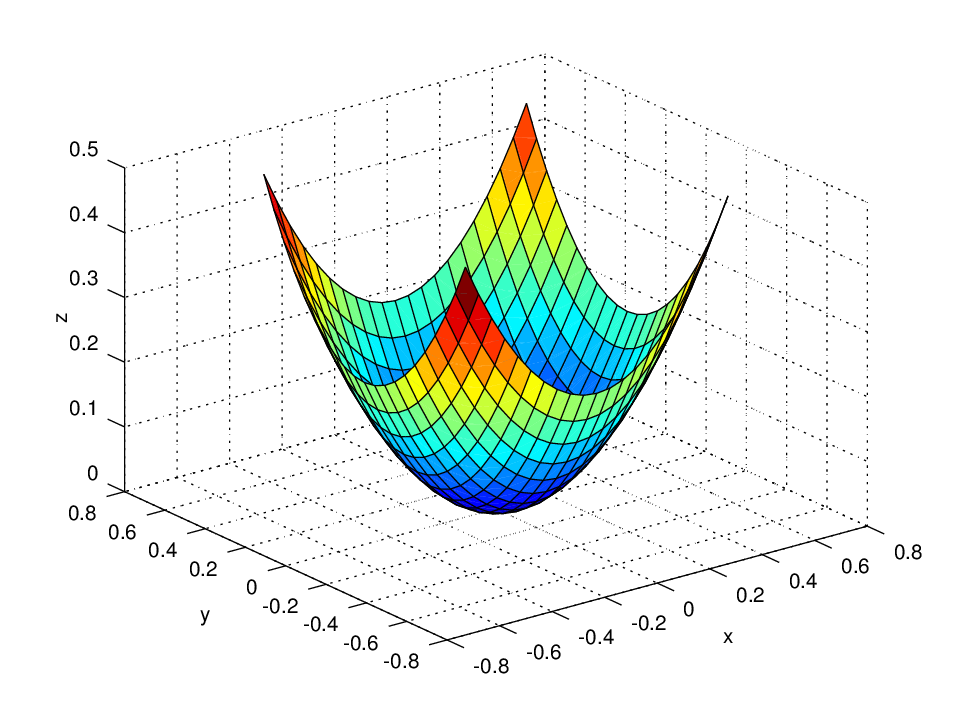
\includegraphics[width=.8\linewidth]{max_bound.png}
            \caption*{$z= f(x,y) = x^2+y^2$.}
        \end{minipage}
    \end{figure}





\subsection{Tilvist útgilda} 

\subsubsection{Setning  \arabic{mycount}}\stepcounter{mycount}
Látum $f$ vera samfellt fall af tveim breytum
skilgreint á lokuðu og takmörkuðu mengi ${\cal D}(f)$.  Fallið $f$
  tekur þá bæði hæsta og lægsta gildi. 




%x


\subsection{Söðulpunktur} 

\subsubsection{Skilgreining  \arabic{mycount}}\stepcounter{mycount}
 Punktur $(x,y)\in  {\cal D}(f)$ sem er ekki
jaðarpunktur kallast {\em \color{red} söðulpunktur} ef $\nabla f(x,y)=\ov$ en $f$
hefur ekki staðbundið útgildi í $(x,y)$.



%x

Dæmi um föll með söðulpunkta.
   \begin{figure}[!h]
        \centering
        \begin{minipage}{.5\textwidth}
            \centering
            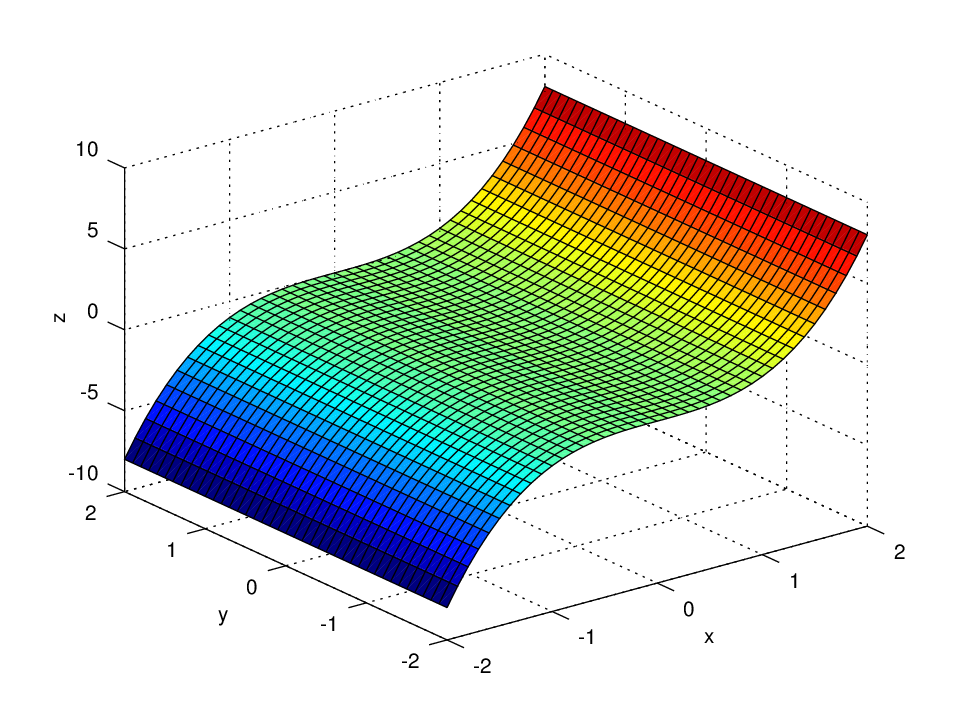
\includegraphics[width=.9\linewidth]{sodull1.png}
            \caption*{$z = f(x,y) = x^3$.}
        \end{minipage}%
        \begin{minipage}{.5\textwidth}
            \centering
            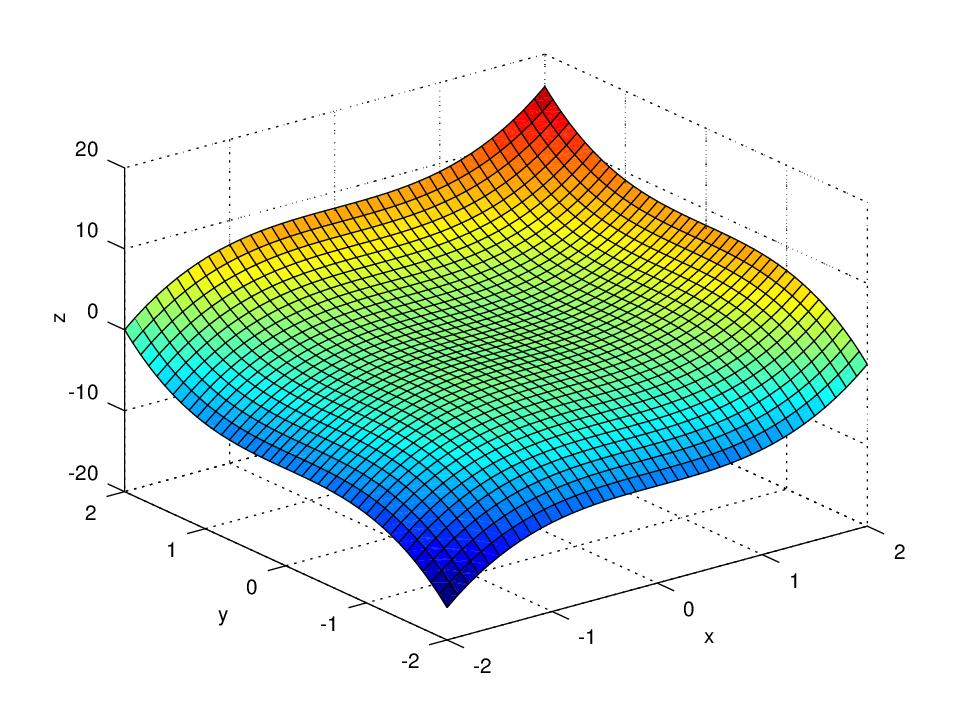
\includegraphics[width=.9\linewidth]{sodull2.png}
            \caption*{$z = f(x,y) = x^3+y^3$.}
        \end{minipage}
        
    \end{figure}



\subsection{Staðbundið útgildi} 

\subsubsection{Upprifjun  \arabic{mycount}}\stepcounter{mycount}
 Látum $f$ vera fall af einni breytistærð og
gerum ráð fyrir að $f'$ sé samfellt fall.  Gerum einnig ráð fyrir að
$f'(a)=0$.  Þá gildir: 

\begin {enumerate}
 \item Ef $f''(a)>0$ þá hefur $f$ staðbundið lággildi í $a$.
 \item  Ef $f''(a)<0$ þá hefur $f$ staðbundið hágildi í $a$.
 \item  Ef $f''(a)=0$ þá gæti verið staðbundið lággildi í $A$, það gæti
     verið staðbundið hágildi í $a$ eða það gætu verið beygjuskil í
     $a$, alltsvo. ekkert hægt að segja. 
 \end {enumerate}




%x


\subsection{Hesse-fylki} 

\subsubsection{Skilgreining  \arabic{mycount}}\stepcounter{mycount}
Látum $f$ vera fall af $n$ breytum $\mathbf{x} = (x_1,x_2,\ldots,x_n)$ og
gerum ráð fyrir að allar 2.~stigs hlutafleiður $f$ séu skilgreindar í
punktinum $\mathbf{x}$.  Skilgreinum  {\em \color{red} Hesse-fylki} $f$ í punktinum
$\mathbf{x}$ sem $n\times n$-fylkið
$${\cal H}(\mathbf{x})=\begin{bmatrix} f_{11}(\mathbf{x})&f_{12}(\mathbf{x}) & \cdots & f_{1n}(\mathbf{x})\\
 f_{21}(\mathbf{x})&f_{22}(\mathbf{x}) & \cdots & f_{2n}(\mathbf{x}) \\
 \vdots & \vdots & \ddots & \vdots & \\
  f_{n1}(\mathbf{x})&f_{n2}(\mathbf{x}) & \cdots & f_{nn}(\mathbf{x})\end{bmatrix}.$$



%x


\subsection{Ferningsform (sjá kafla 10.7 í Adams)} 

\subsubsection{Upprifjun  \arabic{mycount}}\stepcounter{mycount}
{\em \color{red} Ferningsform} $Q$ af $n$-breytum $x_1,x_2,\ldots, x_n$ er einsleit margliða af stigi 2 gefin með 
\begin {equation*}
Q(\mathbf{x}) = \mathbf{x}^T A \mathbf{x}
\end {equation*}
þar sem $A$ er samhverft $n \times n$ fylki með tölu $a_{ij}$ í sæti $(i,j)$ og $\mathbf{x} = [x_1,x_2,\ldots x_n]^T$.







\subsection{Ferningsform} 

\subsubsection{Skilgreining  \arabic{mycount}}\stepcounter{mycount}
Ferningsform $Q$ af $n$-breytum er sagt vera
{\em \color{red} jákvætt ákvarðað}\  (e.~positive definite) ef $Q(\xv)>0$ fyrir
alla vigra $\xv\neq \ov$ í $\Rn$.   

\medskip
Sagt að ferningsformið $Q$ sé
{\em \color{red} neikvætt ákvarðað}\  (e.~negative definite) ef $Q(\xv)<0$ fyrir
alla vigra $\xv\neq \ov$ í $\Rn$.   

\medskip
Síðan er sagt að ferningsformið $Q$ sé
{\em  \color{red} óákvarðað}\  (e.~indefinite) ef $Q(\xv)<0$ fyrir
einhvern vigur $\xv$  og $Q(\yv)>0$ fyrir einhvern vigur
$\yv$. 



%x

\subsubsection{Setning  \arabic{mycount}}\stepcounter{mycount}
 Látum $Q$ vera fernings form  af $n$ breytum og
$A$ samhverft $n\times n$ fylki þannig að $Q(\xv)=\xv^TA\xv$ fyrir
alla vigra $\xv$,
\begin {enumerate}
 \item  Ferningsformið er jákvætt ákvarðað ef og aðeins ef öll eigingildi
    $A$ eru jákvæð.
\item Ferningsformið er neikvætt ákvarðað ef og aðeins ef öll eigingildi
    $A$ eru neikvæð.
\item  Ferningsformið er óákvarðað ef og aðeins ef $A$ hefur bæði jákvæð
     og neikvæð eigingildi.	
\end {enumerate}




%x


\subsection{Staðbundið útgildi} 

\subsubsection{Setning  \arabic{mycount}}\stepcounter{mycount}
 Látum $f$ vera fall af $n$ breytum $\mathbf{x} = (x_1,x_2,\ldots,x_n)$ þannig að allar
1.~og 2.~stigs hlutafleiður $f$ eru samfelldar.  Látum $\mathbf{a}$ vera
innri punkt á skilgreiningarsvæði $f$ og gerum ráð fyrir að $\nabla
f(\mathbf{a})=\ov$.  Þá gildir: Ef ${\cal H}(\mathbf{a})$ er 
\begin {enumerate}
 \item  ...jákvætt ákvarðað þá hefur $f$ staðbundið
     lággildi í $\mathbf{a}$.
\item ...neikvætt ákvarðað þá hefur $f$ staðbundið
     hágildi í $\mathbf{a}$.
\item    ...óákvarðað þá hefur $f$ söðulpunkt í
      $\mathbf{a}$.  
\item ...hvorki jákvætt ákvarðað, neikvætt ákvarðað
      né óákvarðað þá nægja upplýsingarnar sem felast í jöfnunni
      $\nabla f(\mathbf{a})=\ov$ og Hesse-fylkinu ekki til að segja til um
      hvers eðlis stöðupunkturinn $\mathbf{a}$ er.
\end {enumerate}




%x


\subsubsection{Fylgisetning  \arabic{mycount}}\stepcounter{mycount}
Látum $f$ vera fall af tveim breytum þannig að
1.~og 2.~stigs hlutafleiður $f$ eru samfelldar.  Látum $(a,b)$ vera
innri punkt á skilgreiningarsvæði $f$ og gerum ráð fyrir að $\nabla
f(a,b)=\ov$.  Setjum 
$$A=f_{11}(a,b),\qquad\quad B=f_{12}(a,b)=f_{21}(a,b)\qquad\quad
C=f_{22}(a,b).$$ 
Þá gildir:
\begin {enumerate}
 \item  Ef $B^2-AC<0$ og $A>0$  þá hefur $f$
     staðbundið lággildi í $(a,b)$.
 \item  Ef $B^2-AC<0$ og $A<0$ 
 þá hefur $f$ staðbundið
hágildi í $(a,b)$.
 \item   Ef $B^2-AC>0$ 
þá hefur $f$ söðulpunkt í
      $(a,b)$.  
 \item  Ef $B^2-AC=0$ þá er ekkert hægt að segja.  
\end {enumerate}



 
\subsection{Ferningsform}  

\subsubsection{Regla  \arabic{mycount}}\stepcounter{mycount}
Ef $A$ er samhverft $n \times n$ fylki með tölu $a_{ij}$ í sæti $(i,j)$ og
\begin {equation*}
 D_i = \begin{vmatrix}
        a_{11} & a_{12} & \cdots & a_{1i} \\
        a_{21} & a_{22} & \cdots & a_{2i} \\
        \vdots & \vdots & \ddots & \vdots \\ 
        a_{i1} & a_{i2} & \cdots & a_{ii} 
       \end{vmatrix}
\end {equation*}
þá gildir
\begin {enumerate}
 \item Ef $D_i > 0$ fyrir $1\leq i \leq n$ þá er $A$ jákvætt ákvarðað.
 \item Ef $D_i > 0$ fyrir slétt $i$ í $\{1,2,\ldots,n\}$ og $D_i < 0$ fyrir oddatölu $i$ í $\{1,2,\ldots,n\}$ þá er $A$ neikvætt ákvarðað.
 \item Ef $\det(A) = D_n \neq 0$ en hvorki $1$ né $2$ gilda þá er $A$ óákvarðað. 
 \item Ef $\det(A) = 0$ þá er $A$ hvorki jákvætt né neikvætt ákvarðað en getur verið óákvarðað.
\end {enumerate}




\subsection{Útgildi falla þar sem breytur uppfylla skorðujöfnur} 

\subsubsection{Sértækar aðferðir  \arabic{mycount}}\stepcounter{mycount}
Finna skal útgildi falls $f(x,y)$ þegar skilgreiningarsvæði $f$ er mengi þeirra punkta $(x,y)$ sem uppfylla jöfnu $g(x,y)=0$.  


\begin {enumerate}
 \item Er mögulegt að einangra $x$ eða $y$ í jöfnunni $g(x,y)=0$?  
 
 \medskip
 \begin {itemize}
  \item [] Ef hægt er að einangra $y$ og rita $y=h(x)$ þá snýst verkefnið nú um að finna útgildi falls $f(x,h(x))$ af einni breytu $x$.

 \end {itemize}
 \item  Er hægt að stika ferilinn $g(x,y)=0$?  
 
 \begin {itemize}
  \item [] Ef $\rv$ er stikun á
     ferlinum þá þurfum við að leita að útgildum fallsins $f(\rv(t))$ þar sem
     er bara ein breyta.  
 \end {itemize}

\end {enumerate}








\subsubsection{Dæmi}
 \begin {figure}[h!]
 \centering
            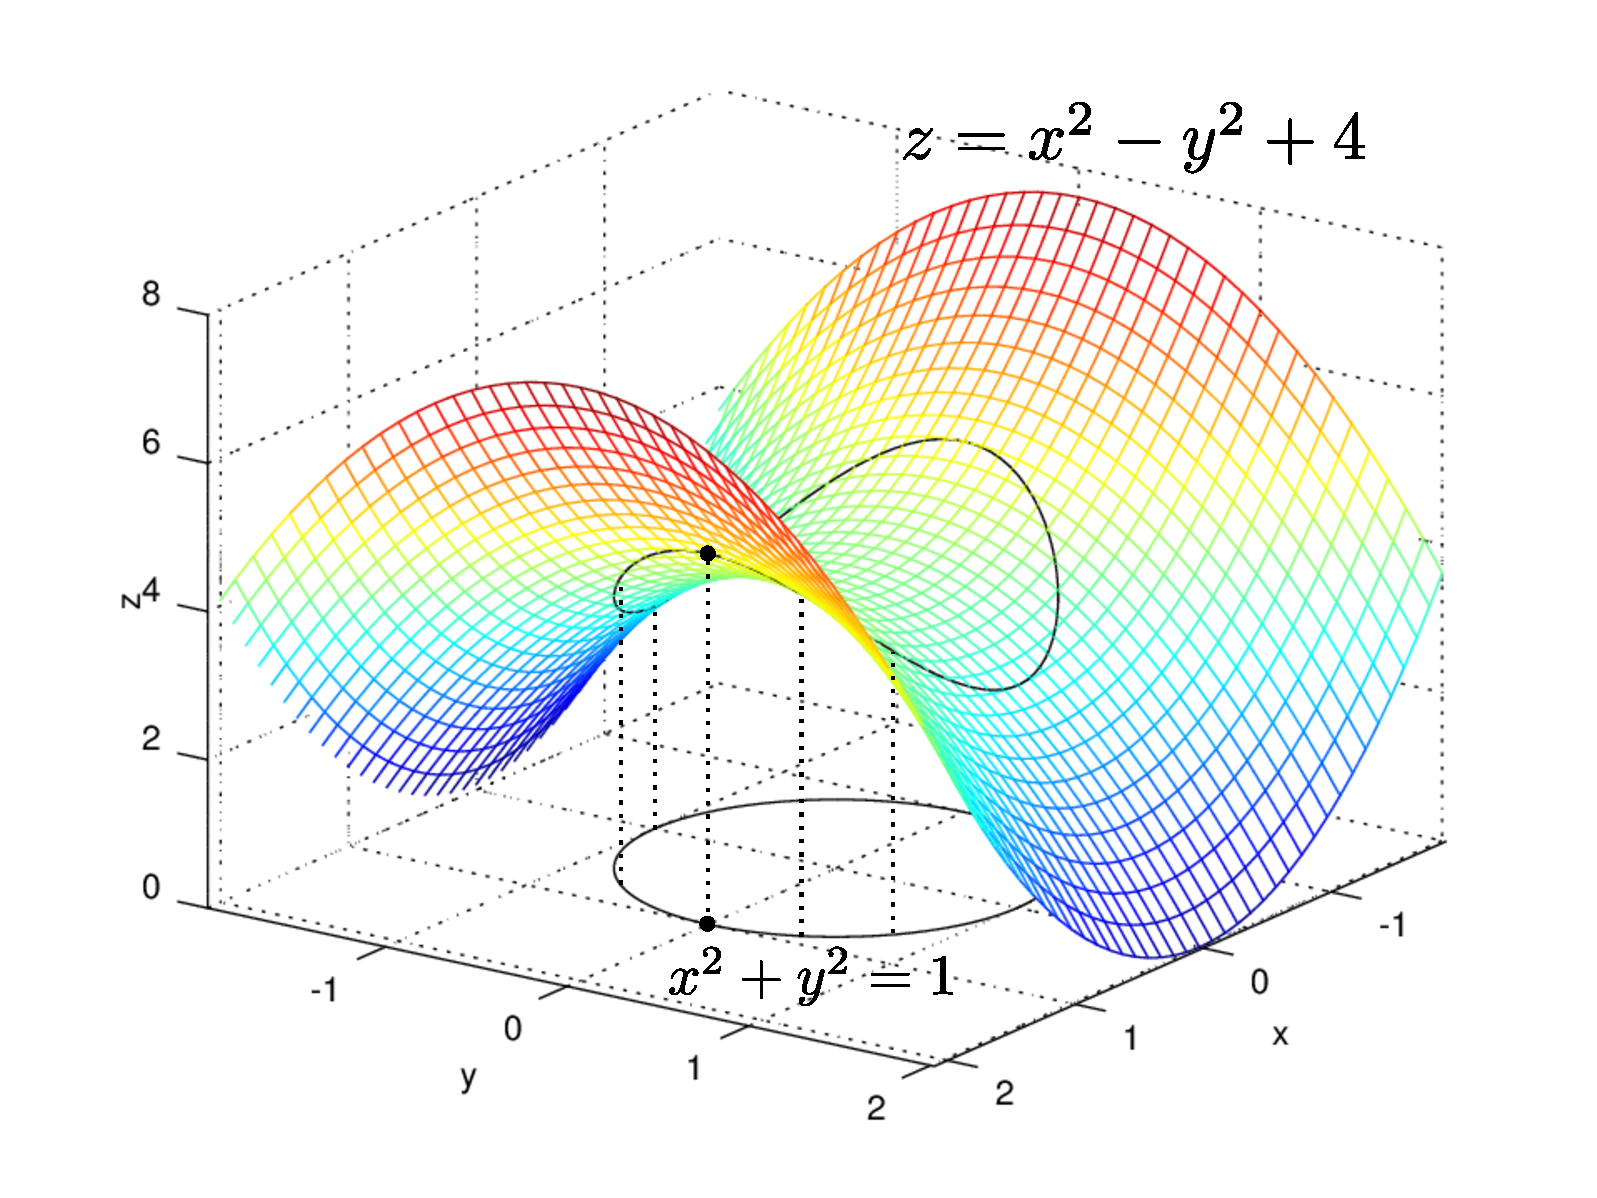
\includegraphics[width=.7\linewidth]{constraint.pdf}
            \caption*{Hver eru hæstu og lægstu gildi fallsins $f(x,y) = x^2-y^2+4$ á menginu $\{(x,y)~|~x^2+y^2=1\}$?}
\end {figure}




 


\subsection{Útgildi falla þar sem breytur uppfylla skorðujöfnur} 

\subsubsection{Setning  \arabic{mycount}}\stepcounter{mycount}
Látum $f$ og $g$ vera föll sem eru bæði
diffranleg í punktinum $P_0=(x_0,y_0)$ sem liggur á ferlinum
$g(x,y)=0$, og er ekki endapunktur ferilsins.  Gerum ráð fyrir að
$\nabla g(x_0,y_0)\neq \ov$.  Gerum líka ráð fyrir að ef við einskorðum fallið $f$ við ferilinn $g(x,y)=0$ þá hafi $f$ staðbundið útgildi í $P_0$.  Þá eru stiglarnir $\nabla f(x_0,y_0)$ og $\nabla g(x_0,y_0)$ samsíða.


\begin {figure}[h!]
 \centering
            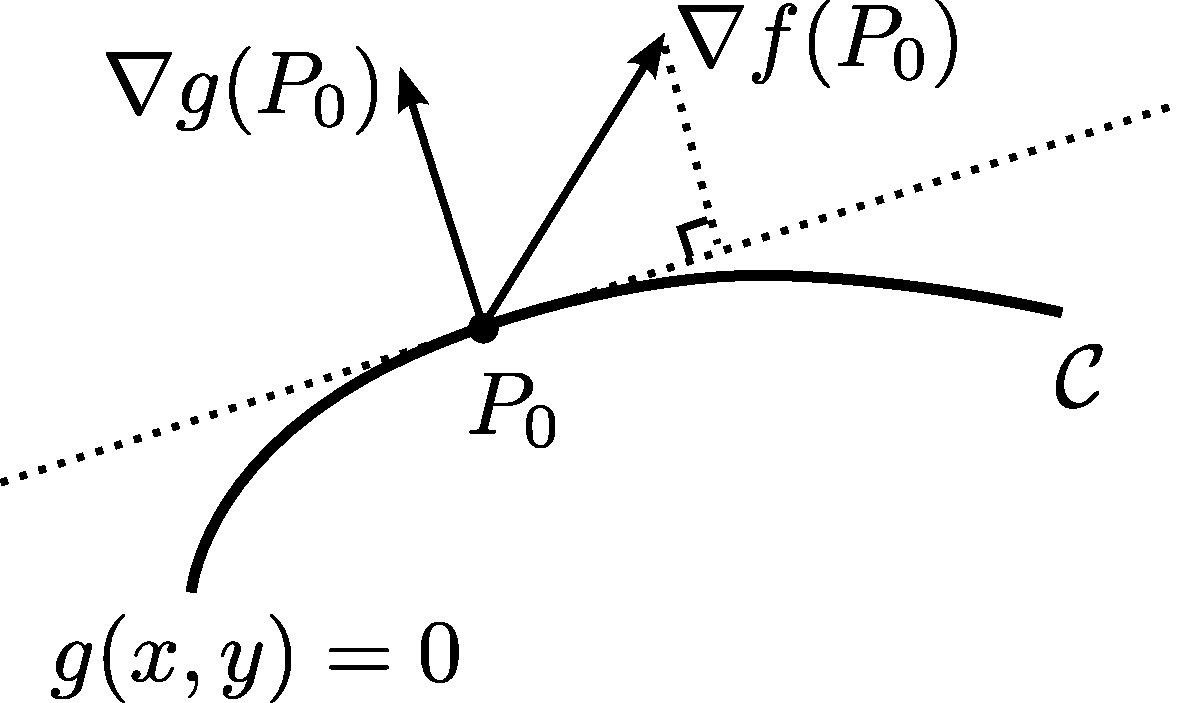
\includegraphics[width=.4\linewidth]{lagrange1}
            \caption*{Ef stiglarnir $\nabla g(P_0)$ og $\nabla f(P_0)$ eru ekki samsíða þá vex $f$ eða minnkar þegar farið er eftir $\mathcal{C}$ út frá punktinum $P_0$.}
\end {figure}



\subsection{Lagrange-margfaldarar} 

\subsubsection{Reikniaðferð  \arabic{mycount}}\stepcounter{mycount}
  Finna skal útgildi falls $f(x,y)$ þegar skilgreiningarsvæði $f$ er mengi þeirra punkta $(x,y)$ sem uppfylla jöfnu $g(x,y)=0$.  

\medskip
Búum til {\em Lagrange-fallið}
$$L(x,y,\lambda)=f(x,y)+\lambda g(x,y).$$
Stöðupunktar $L$, þ.e.a.s.~punktar $(x_0,y_0,\lambda_0)$ þar sem $\nabla L(x_0,y_0,\lambda_0)=\ov$, gefa mögulega punkta $(x_0,y_0)$ þar sem $f$ tekur útgildi.

\medskip
Þessir punktar finnast með því að leysa jöfnuhneppið
\begin{align*}
f_1(x,y)+\lambda g_1(x,y)&=0\\
f_2(x,y)+\lambda g_2(x,y)&=0\\
g(x,y)&=0.
\end{align*}

Talan $\lambda$ nefnist \emph{Lagrange-margfaldari}.



\subsubsection{Regla  \arabic{mycount}}\stepcounter{mycount}
Finna skal útgildi falls $f(x,y)$ þegar skilgreiningarsvæði $f$ er mengi þeirra punkta $(x,y)$ sem uppfylla jöfnu $g(x,y)=0$.  

Athuga þarf punkta sem uppfylla eitt af eftirfarandi skilyrðum:

\begin {enumerate}
 \item Stöðupunktar $L(x,y,\lambda)$.
\item Punktar $(x,y)$ þar sem $\nabla g(x,y)=\ov$.
\item  Punktar $(x,y)$ þar sem annar eða báðir stiglanna $\nabla
      g(x,y)$ og $\nabla f(x,y)$ eru ekki skilgreindir. 
\item ,,Endapunktar\lq\lq\ ferilsins $g(x,y)=0$.
 \end {enumerate}





\subsubsection{Reikniaðferð  \arabic{mycount}}\stepcounter{mycount}
Finna skal útgildi falls $f(x,y,z)$ þegar skilgreiningarsvæði $f$ er mengi þeirra punkta $(x,y,z)$ sem uppfylla jöfnurnar $g(x,y,z)=0$ og $h(x,y,z)=0$.  

Búum til Lagrange-fallið
$$L(x,y,z,\lambda,\mu)=f(x,y,z)+\lambda g(x,y,z)+\mu h(x,y,z).$$
Stöðupunktar $L$, þ.e.a.s.~punktar $(x_0,y_0,z_0,\lambda_0,\mu_0)$ þar sem $\nabla L(x_0,y_0,z_0,\lambda_0,\mu_0)=\ov$ gefa mögulega punkta $(x_0,y_0,z_0)$ þar sem $f$ tekur útgildi.

Þessir punktar finnast með því að leysa jöfnuhneppið
\begin{align*}
f_1(x,y,z)+\lambda g_1(x,y,z)+\mu h_1(x,y,z)&=0\\
f_2(x,y,z)+\lambda g_2(x,y,z)+\mu h_2(x,y,z)&=0\\
f_3(x,y,z)+\lambda g_3(x,y,z)+\mu h_3(x,y,z)&=0\\
g(x,y,z)&=0\\
h(x,y,z)&=0.
\end{align*}







\end{document}
